%%%%%%%%%%%%%%%%%%%%%%%%%%%%%%%%%%%%%%%%%%%%%%%%%%%%%%%%%%%%%%%%%%%%%%%%%%%%%%%%
%2345678901234567890123456789012345678901234567890123456789012345678901234567890
%        1         2         3         4         5         6         7         8

\documentclass[letterpaper, 10 pt, conference]{ieeeconf}  % Comment this line out if you need a4paper

%\documentclass[a4paper, 10pt, conference]{ieeeconf}      % Use this line for a4 paper

\IEEEoverridecommandlockouts                              % This command is only needed if 
                                                          % you want to use the \thanks command

\overrideIEEEmargins                                      % Needed to meet printer requirements.

% See the \addtolength command later in the file to balance the column lengths
% on the last page of the document

% The following packages can be found on http:\\www.ctan.org
\usepackage{graphicx} % for pdf, bitmapped graphics files
%\usepackage{epsfig} % for postscript graphics files
%\usepackage{mathptmx} % assumes new font selection scheme installed
%\usepackage{times} % assumes new font selection scheme installed
\usepackage{amsmath} % assumes amsmath package installed
\usepackage{amssymb}  % assumes amsmath package installed
\usepackage{multicol}

\title{\LARGE \bf
Proposal for Analysis of Security In a Modern Processor
}


\author{Justin Cox and Tyler Travis
\\ \small{Department of Electrical and Computer Engineering}
\\ \small{Utah State University}
\\ \small{Logan, Utah 84322}
\\ \small{email: justin.n.cox@gmail.com, tyler.travis@aggiemail.usu.edu}
}


\begin{document}



\maketitle
\thispagestyle{empty}
\pagestyle{empty}


%%%%%%%%%%%%%%%%%%%%%%%%%%%%%%%%%%%%%%%%%%%%%%%%%%%%%%%%%%%%%%%%%%%%%%%%%%%%%%%%
\begin{abstract}

Hardware security is an ever increasing area of study since exploits have been found on computer systems. It has been found that attackers are able to look at the memory of a system to see what is being processed. This paper proposes adding an extra level of security between the memory and the pipeline. This layer of security would encrypt data headed to memory and decrypt the data headed to the pipeline making the data held in memory incomprehensible to an attacker. To make the added cryptographic system more secure, research will be done on the benefits of utilizing a Physically Unclonable Function (PUF). Further analysis will be done on how this will affect the processor's performance.

\emph{Index Terms}---encryption, decryption, security, pipeline, PUF.

\end{abstract}

%%%%%%%%%%%%%%%%%%%%%%%%%%%%%%%%%%%%%%%%%%%%%%%%%%%%%%%%%%%%%%%%%%%%%%%%%%%%%%%%
\section{INTRODUCTION}

Over the years, there have been many advancements made to computer systems and architecture. These advancements have been primarily focused on improving performance and power consumption. As a result, the security of these architectures has been neglected. Malicious attacks on computer systems are becoming more common and as a result, there is greater need for more secure systems.

The optimal solution to this problem is to completely redevelop the architectures with security as a top priority. However this option is not very practical as it would be far too expensive to replace the current processors and there is a need to support legacy machines. Therefore, we propose to create security modules that can be added to current processor architecture.

This paper shows the authors' process of developing a DES cryptography module designed to be inserted into the gem5 simulation software.  The paper also shows how a PUF can be used to increase the security of the DES module.  The results of the architecture's performance with the added security module will be simulated and the results will be given. 

%%%%%%%%%%%%%%%%%%%%%%%%%%%%%%%%%%%%%%%%%%%%%%%%%%%%%%%%%%%%%%%%%%%%%%%%%%%%%%%%
\section{BACKGROUND}

Computer security is becoming more important as more systems and devices are being compromised.  In particular, there has been an increased number of attacks focused on stealing information stored in memory on computers and servers.  This information can be encrypted when not in use, but currently there are very few solutions that allow the computer architecture to work with the encrypted data.  As a result, when the architecture is running, the data stored in memory is vulnerable to attackers.

Previous research has been done on the development and implementation of secure processors [1].  Similar to the previous research done, this paper will focus on data encryption and decryption and the toll it takes on processor performance.  The objective is to provide as much security as possible without reducing the performance heavily.

%%%%%%%%%%%%%%%%%%%%%%%%%%%%%%%%%%%%%%%%%%%%%%%%%%%%%%%%%%%%%%%%%%%%%%%%%%%%%%%%
\section{TECHNIQUE}

The following subsections will describe the techniques used to supply current computer architecture with more data security. The first subsection will describe how the data will be protected by cryptography. The last section will describe how the cyptograhic modules will be improved using a PUF.

\subsection{Encryption and Decryption of Data}

The memory can be modified by an attacker and as a result the attacker is able to change the execution flow of a program.  Since the data is not encrypted, the attacker is also able to steal important information that may be contained in memory. Therefore to prevent the attacker from knowing where to modify or read the data, it is important for the CPU to encrpyt data being stored into memory. Initially, we will encrypt memory that is stored in registers, cache, RAM, and virtual memory [1]. If the performance decreases significantly, encryption will be excluded from the registers and/or cache. Assuming the pipeline is trusted, data being pushed into the pipeline will be decrypted.

These encryption and decryption modules will be built and inserted into the gem5 source code.

\subsection{Data Encryption Standard (DES)}

The type of encryption used for the module will be DES.  Although DES is not the current encryption standard and is not as secure as the Advanced Encryption Standard AES, DES will allow better processor performance while still making the data more secure.

A brief overview of DES will be given so that the reader has a better understanding of how encryption could take a toll on processor performance.  If the reader would like an in-depth understanding of DES, it is recommended that the reader look to other sources.

The DES algorithm takes a 64-bit plain text input.  It is then run through an initial permutation that outputs 56-bits when are then split into two halves.  The data goes through sixteen rounds that each have a sub-key that is generated for each round based on the original 64-bit DES key.  After the sixteenth round, the output is run through a finial permutation and the algorithm outputs a 64-bit encrypted cipher text.  The rounds are illustrated in Figure 1.

\begin{figure}[thpb]
	\centering
	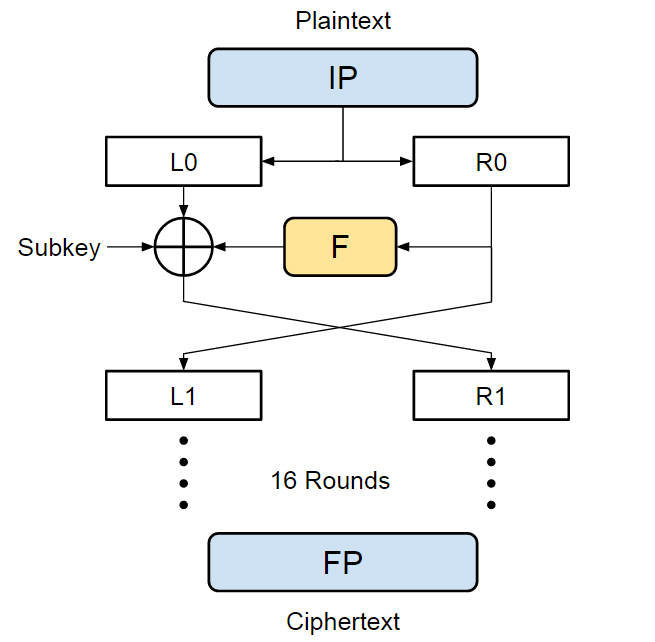
\includegraphics[scale=.50]{DesRounds}
    \caption{An illustration of the sixteen round DES algorithm.}
\end{figure}

During each round, the left 32-bit halve is XORed with the sub key corresponding to the current round as well as the output of the F-function.  The inside functionality of the F-function is illustrated in Figure 2. The output of the XOR is used as the next round's right halve and the next round's left halve is the previous round's right halve.

\begin{figure}[thpb]
	\centering
	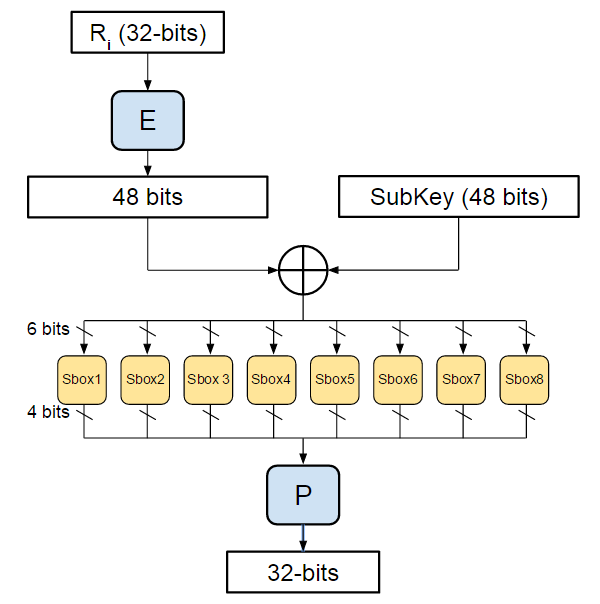
\includegraphics[scale=.50]{Ffunction}
    \caption{An illustration of the F-function}
\end{figure}


\subsection{Physically Unclonable Function (PUF)}

A PUF is used to generate secrets extracted from a physical device due to manufacturing differences. This uniqueness can be used for more secure key generation for encryption/decryption [2]. Since the PUF output is generated by a physical device, a predetermined secret will be used to simulate the PUF output. 

\section{METHODOLOGY}

\subsection{Benchmarking and Performance}

The simulator that this project will use is gem5. The security modules will be added on to several different processor benchmarks found in gem5. A chosen application will be run on all benchmarks without the added security modules and again with the added security modules. The performance will be compared between the results. The gem5 simulator will be ran with using the out of order model, or O3. Some of the benchmarks the team are looking at running are:

\begin{multicols}{2}
\begin{itemize}
\item bzip2
\item gcc
\item bwaves
\item mcf
\item gobmk
\item hmmer
\item GemsFDTD
\item libquantum
\item tonto
\item omnetpp
\end{itemize}
\end{multicols}

\section{PROGRESS MADE}

Over the last few weeks, the team has been working on a DES implementation in C++. The program is able to encrypt and decrypt data in blocks of 16 bytes. Current bottlenecks that the team is facing is how to implement the DES mdoule into the gem5 source code. In the initial design, the DES module will have an interface between the registers, caches, RAM, and disk and the CPU. Finding these locations and directing their output to the DES module and sending the data to the right location will be a challenge. 

The next area the team needs to work on is implementation of a pseudo-PUF for secret key generation. Since a PUF is based on physical imperfections at a silicon level, this can't really be modeled in software. The team needs to either build a database of sampled PUF outputs to simulate a PUF, or settle with a pseudo random number generator. Since this is only a proof of concept project, the actual security of this device is negilible. Next, the team needs to find a way to put
this together with the gem5 simulator. 

In the future, the team may decide to use different CPU models to see how the DES module effects the overall performance. Some ideas the team had are multi-core and in-order CPU models. 

\addtolength{\textheight}{-12cm}   % This command serves to balance the column lengths
                                  % on the last page of the document manually. It shortens
                                  % the textheight of the last page by a suitable amount.
                                  % This command does not take effect until the next page
                                  % so it should come on the page before the last. Make
                                  % sure that you do not shorten the textheight too much.

%%%%%%%%%%%%%%%%%%%%%%%%%%%%%%%%%%%%%%%%%%%%%%%%%%%%%%%%%%%%%%%%%%%%%%%%%%%%%%%%



%%%%%%%%%%%%%%%%%%%%%%%%%%%%%%%%%%%%%%%%%%%%%%%%%%%%%%%%%%%%%%%%%%%%%%%%%%%%%%%%



%%%%%%%%%%%%%%%%%%%%%%%%%%%%%%%%%%%%%%%%%%%%%%%%%%%%%%%%%%%%%%%%%%%%%%%%%%%%%%%%

%\section*{ACKNOWLEDGMENT}

%The author would like to thank his instructor Dr. Rajnikant Sharma %for his help in understanding control concepts.




%%%%%%%%%%%%%%%%%%%%%%%%%%%%%%%%%%%%%%%%%%%%%%%%%%%%%%%%%%%%%%%%%%%%%%%%%%%%%%%%




\begin{thebibliography}{99}

\bibitem{c1} G. Edward Suh, C. W. O'Donnel, I. Sachdev, and S Devadas. Design and Implementation of the AEGIS Single-Chip Secure Processor Using Physical Random Functions. \emph{Proceedings of the 32nd annual international symposium on Computer Architecture}, 2005.
\bibitem{c2} M. Deutschman, "Cryptographic Applications with Physically Unclonable Functions," M.S. Thesis, Inst. Mathematics, Alpen-Adria-Universit\"{a}t Klagenfurt, Klagenfurt, Austria, 2010.
 

\end{thebibliography}

\end{document}
